\documentclass[12pt]{article}
\usepackage[utf8]{inputenc}
\usepackage{geometry}
\geometry{a4paper, margin=1in}
\usepackage{graphicx}
\usepackage{booktabs}
\usepackage{tabularx}
\usepackage{xcolor}
\usepackage{amsmath}
\usepackage{hyperref}

\title{
  \textbf{Tugas Algoritma Genetika --- Studi Kasus TSP} \\
  \vspace{0.5em}
  \large \textbf{Mata Kuliah:} Kecerdasan Komputasional \\
  \large \textbf{Dosen Pengampu:} [Nama Dosen Anda]
}
\author{
  \textbf{Kelompok 6} \\
  1. Rizki Pratama Sunarko (240411100181) \\
  2. Ainur Suharyanto (240411100154)\\
  3. Wahyu Ari Ananda Fitrotul Huda (240411100148)\\
}
\date{}

\begin{document}
\maketitle
\vspace{5em}
\section{Pendahuluan}
Studi kasus ini menyelesaikan \textit{Traveling Salesperson Problem} (TSP) menggunakan Algoritma Genetika, bukan optimasi fungsi $x^2$. Data yang diproses berupa koordinat dari 15 kota di Amerika Serikat. Algoritma genetika diimplementasikan dengan spesifikasi:

\begin{itemize}
    \item \textbf{Seleksi}: Rank Selection
    \item \textbf{Crossover}: Order Crossover (OX)
    \item \textbf{Mutasi}: Inversion Mutation
    \item \textbf{Elitism}: Mempertahankan individu terbaik di setiap generasi
    \item \textbf{Jumlah Iterasi}: 5
    \item \textbf{Ukuran Populasi}: 4 Kromosom (untuk mempermudah perhitungan manual)
    \item \textbf{Peluang Crossover ($P_c$)}: 0.8
    \item \textbf{Peluang Mutasi ($P_m$)}: 0.2
\end{itemize}
\vspace{15em}

\section{Data Kota}
Berikut adalah daftar 15 kota beserta indeksnya yang digunakan sebagai representasi gen pada kromosom.

\begin{table}[h!]\centering
\begin{tabular}{clcc}
\toprule
\textbf{Indeks} & \textbf{Kota} & \textbf{Latitude} & \textbf{Longitude} \\
\midrule
0 & Denver & 39.7420 & -104.9915 \\
1 & Colorado Springs & 38.8461 & -104.8006 \\
2 & Telluride & 37.9375 & -107.8123 \\
3 & Las Vegas & 36.1146 & -115.1728 \\
4 & Grand Canyon & 36.0565 & -112.1251 \\
5 & Yellowstone NP & 44.4237 & -110.5885 \\
6 & Mount Rushmore & 43.9686 & -103.3818 \\
7 & Seattle & 47.6080 & -122.3352 \\
8 & Redwood NP & 41.2131 & -124.0046 \\
9 & San Diego & 32.7157 & -117.1610 \\
10 & Los Angeles & 34.0522 & -118.2437 \\
11 & Mount Hood NF & 45.4543 & -121.9331 \\
12 & Santa Fe & 35.6915 & -105.9442 \\
13 & Chicago & 41.8818 & -87.6232 \\
14 & New York City & 40.7306 & -73.9352 \\
\bottomrule
\end{tabular}
\end{table}


\section{Perhitungan Manual (5 Iterasi)}
\subsection*{Iterasi 1}
\textbf{1. Evaluasi Fitness}\\$Fitness = 1 / Total Jarak$
\begin{itemize}
\item K1: [8, 13, 7, 6, 14, 12, 5, 2, 9, 3, 4, 11, 0, 1, 10] $\rightarrow$ Jarak: 243.38, Fitness: 0.004109
\item K2: [2, 12, 9, 7, 4, 6, 5, 10, 13, 8, 11, 3, 1, 14, 0] $\rightarrow$ Jarak: 237.92, Fitness: 0.004203
\item K3: [7, 8, 3, 11, 10, 14, 1, 13, 5, 6, 2, 0, 12, 4, 9] $\rightarrow$ Jarak: 206.82, Fitness: 0.004835
\item K4: [12, 8, 6, 2, 10, 11, 3, 14, 7, 0, 4, 9, 13, 5, 1] $\rightarrow$ Jarak: 270.74, Fitness: 0.003694
\end{itemize}
\vspace{0.5cm}\textbf{2. Rank Selection}\\Kromosom diurutkan berdasarkan fitness (tertinggi ke terendah) dan diberi rank:
\begin{table}[h!]\centering\begin{tabular}{ccccc}\toprule Rank & Kromosom & Probabilitas & Kumulatif Probabilitas \\ \midrule
4 & [7, 8, 3, 11, 10, 14, 1, 13, 5, 6, 2, 0, 12, 4, 9] & 0.40 & 0.40 \\
3 & [2, 12, 9, 7, 4, 6, 5, 10, 13, 8, 11, 3, 1, 14, 0] & 0.30 & 0.70 \\
2 & [8, 13, 7, 6, 14, 12, 5, 2, 9, 3, 4, 11, 0, 1, 10] & 0.20 & 0.90 \\
1 & [12, 8, 6, 2, 10, 11, 3, 14, 7, 0, 4, 9, 13, 5, 1] & 0.10 & 1.00 \\
\bottomrule\end{tabular}\end{table}
Terpilih Parent 1: [2, 12, 9, 7, 4, 6, 5, 10, 13, 8, 11, 3, 1, 14, 0]\\
Terpilih Parent 2: [8, 13, 7, 6, 14, 12, 5, 2, 9, 3, 4, 11, 0, 1, 10]\\

\vspace{0.5cm}
\noindent\textbf{3. Crossover (Order Crossover / OX)}\\Menghasilkan keturunan menggunakan probabilitas crossover $P_c = 0.8$.\\
\textbf{Elitism diterapkan}: Kromosom terbaik diteruskan tanpa diubah: [7, 8, 3, 11, 10, 14, 1, 13, 5, 6, 2, 0, 12, 4, 9]\\
\textbullet\ $r\_cross = 0.05 \le 0.8$: Crossover pada titik 3 hingga 12.\\ Anak dihasilkan: [2, 9, 0, 7, 4, 6, 5, 10, 13, 8, 11, 3, 1, 14, 12]\\
\textbullet\ $r\_cross = 0.29 \le 0.8$: Crossover pada titik 1 hingga 13.\\ Anak dihasilkan: [0, 12, 9, 7, 4, 6, 5, 10, 13, 8, 11, 3, 1, 14, 2]\\
\textbullet\ $r\_cross = 0.23 \le 0.8$: Crossover pada titik 1 hingga 6.\\ Anak dihasilkan: [14, 12, 9, 7, 4, 6, 5, 2, 3, 11, 0, 1, 10, 8, 13]\\

\vspace{0.5cm}
\noindent\textbf{4. Mutasi (Inversion Mutation)}\\Mengecek kromosom baru (kecuali individu elit) untuk mutasi dengan $P_m = 0.2$.\\
\textbullet\ Anak 2 ($r\_mut = 0.28 > 0.2$): Tidak terjadi mutasi.\\
\textbullet\ Anak 3 ($r\_mut = 0.64 > 0.2$): Tidak terjadi mutasi.\\
\textbullet\ Anak 4 ($r\_mut = 0.36 > 0.2$): Tidak terjadi mutasi.\\
\vspace{1cm}
\subsection*{Iterasi 2}
\textbf{1. Evaluasi Fitness}\\$Fitness = 1 / Total Jarak$
\begin{itemize}
\item K1: [7, 8, 3, 11, 10, 14, 1, 13, 5, 6, 2, 0, 12, 4, 9] $\rightarrow$ Jarak: 206.82, Fitness: 0.004835
\item K2: [2, 9, 0, 7, 4, 6, 5, 10, 13, 8, 11, 3, 1, 14, 12] $\rightarrow$ Jarak: 252.34, Fitness: 0.003963
\item K3: [0, 12, 9, 7, 4, 6, 5, 10, 13, 8, 11, 3, 1, 14, 2] $\rightarrow$ Jarak: 242.08, Fitness: 0.004131
\item K4: [14, 12, 9, 7, 4, 6, 5, 2, 3, 11, 0, 1, 10, 8, 13] $\rightarrow$ Jarak: 212.75, Fitness: 0.004700
\end{itemize}
\vspace{0.5cm}\textbf{2. Rank Selection}\\Kromosom diurutkan berdasarkan fitness (tertinggi ke terendah) dan diberi rank:
\begin{table}[h!]\centering\begin{tabular}{ccccc}\toprule Rank & Kromosom & Probabilitas & Kumulatif Probabilitas \\ \midrule
4 & [7, 8, 3, 11, 10, 14, 1, 13, 5, 6, 2, 0, 12, 4, 9] & 0.40 & 0.40 \\
3 & [14, 12, 9, 7, 4, 6, 5, 2, 3, 11, 0, 1, 10, 8, 13] & 0.30 & 0.70 \\
2 & [0, 12, 9, 7, 4, 6, 5, 10, 13, 8, 11, 3, 1, 14, 2] & 0.20 & 0.90 \\
1 & [2, 9, 0, 7, 4, 6, 5, 10, 13, 8, 11, 3, 1, 14, 12] & 0.10 & 1.00 \\
\bottomrule\end{tabular}\end{table}
Terpilih Parent 1: [7, 8, 3, 11, 10, 14, 1, 13, 5, 6, 2, 0, 12, 4, 9]\\
Terpilih Parent 2: [7, 8, 3, 11, 10, 14, 1, 13, 5, 6, 2, 0, 12, 4, 9]\\

\vspace{0.5cm}
\noindent\textbf{3. Crossover (Order Crossover / OX)}\\Menghasilkan keturunan menggunakan probabilitas crossover $P_c = 0.8$.\\
\textbf{Elitism diterapkan}: Kromosom terbaik diteruskan tanpa diubah: [7, 8, 3, 11, 10, 14, 1, 13, 5, 6, 2, 0, 12, 4, 9]\\
\textbullet\ $r\_cross = 0.27 \le 0.8$: Crossover pada titik 10 hingga 14.\\ Anak dihasilkan: [7, 8, 3, 11, 10, 14, 1, 13, 5, 6, 2, 0, 12, 4, 9]\\
\textbullet\ $r\_cross = 0.65 \le 0.8$: Crossover pada titik 9 hingga 10.\\ Anak dihasilkan: [7, 8, 3, 11, 10, 14, 1, 13, 5, 6, 2, 0, 12, 4, 9]\\
\textbullet\ $r\_cross = 0.17 \le 0.8$: Crossover pada titik 3 hingga 11.\\ Anak dihasilkan: [7, 8, 3, 11, 10, 14, 1, 13, 5, 6, 2, 0, 12, 4, 9]\\

\vspace{0.5cm}
\noindent\textbf{4. Mutasi (Inversion Mutation)}\\Mengecek kromosom baru (kecuali individu elit) untuk mutasi dengan $P_m = 0.2$.\\
\textbullet\ Anak 2 ($r\_mut = 0.16 \le 0.2$): Mutasi inversi segmen dari titik 4 hingga 6.\\ Hasil: [7, 8, 3, 11, 1, 14, 10, 13, 5, 6, 2, 0, 12, 4, 9]\\
\textbullet\ Anak 3 ($r\_mut = 0.99 > 0.2$): Tidak terjadi mutasi.\\
\textbullet\ Anak 4 ($r\_mut = 0.64 > 0.2$): Tidak terjadi mutasi.\\
\vspace{1cm}
\subsection*{Iterasi 3}
\textbf{1. Evaluasi Fitness}\\$Fitness = 1 / Total Jarak$
\begin{itemize}
\item K1: [7, 8, 3, 11, 10, 14, 1, 13, 5, 6, 2, 0, 12, 4, 9] $\rightarrow$ Jarak: 206.82, Fitness: 0.004835
\item K2: [7, 8, 3, 11, 1, 14, 10, 13, 5, 6, 2, 0, 12, 4, 9] $\rightarrow$ Jarak: 227.36, Fitness: 0.004398
\item K3: [7, 8, 3, 11, 10, 14, 1, 13, 5, 6, 2, 0, 12, 4, 9] $\rightarrow$ Jarak: 206.82, Fitness: 0.004835
\item K4: [7, 8, 3, 11, 10, 14, 1, 13, 5, 6, 2, 0, 12, 4, 9] $\rightarrow$ Jarak: 206.82, Fitness: 0.004835
\end{itemize}
\vspace{0.5cm}\textbf{2. Rank Selection}\\Kromosom diurutkan berdasarkan fitness (tertinggi ke terendah) dan diberi rank:
\begin{table}[h!]\centering\begin{tabular}{ccccc}\toprule Rank & Kromosom & Probabilitas & Kumulatif Probabilitas \\ \midrule
4 & [7, 8, 3, 11, 10, 14, 1, 13, 5, 6, 2, 0, 12, 4, 9] & 0.40 & 0.40 \\
3 & [7, 8, 3, 11, 10, 14, 1, 13, 5, 6, 2, 0, 12, 4, 9] & 0.30 & 0.70 \\
2 & [7, 8, 3, 11, 10, 14, 1, 13, 5, 6, 2, 0, 12, 4, 9] & 0.20 & 0.90 \\
1 & [7, 8, 3, 11, 1, 14, 10, 13, 5, 6, 2, 0, 12, 4, 9] & 0.10 & 1.00 \\
\bottomrule\end{tabular}\end{table}
Terpilih Parent 1: [7, 8, 3, 11, 10, 14, 1, 13, 5, 6, 2, 0, 12, 4, 9]\\
Terpilih Parent 2: [7, 8, 3, 11, 10, 14, 1, 13, 5, 6, 2, 0, 12, 4, 9]
\vspace{0.5cm}

\vspace{0.5cm}
\noindent\textbf{3. Crossover (Order Crossover / OX)}\\Menghasilkan keturunan menggunakan probabilitas crossover $P_c = 0.8$.\\
\textbf{Elitism diterapkan}: Kromosom terbaik diteruskan tanpa diubah: [7, 8, 3, 11, 10, 14, 1, 13, 5, 6, 2, 0, 12, 4, 9]\\
\textbullet\ $r\_cross = 0.84 > 0.8$: Tidak terjadi crossover. Anak menyalin Parent 1.\\
\textbullet\ $r\_cross = 0.78 \le 0.8$: Crossover pada titik 3 hingga 13.\\ Anak dihasilkan: [7, 8, 3, 11, 10, 14, 1, 13, 5, 6, 2, 0, 12, 4, 9]\\
\textbullet\ $r\_cross = 0.03 \le 0.8$: Crossover pada titik 5 hingga 6.\\ Anak dihasilkan: [7, 8, 3, 11, 10, 14, 1, 13, 5, 6, 2, 0, 12, 4, 9]\\

\vspace{0.5cm}
\noindent\textbf{4. Mutasi (Inversion Mutation)}\\Mengecek kromosom baru (kecuali individu elit) untuk mutasi dengan $P_m = 0.2$.\\
\textbullet\ Anak 2 ($r\_mut = 0.27 > 0.2$): Tidak terjadi mutasi.\\
\textbullet\ Anak 3 ($r\_mut = 0.21 > 0.2$): Tidak terjadi mutasi.\\
\textbullet\ Anak 4 ($r\_mut = 0.94 > 0.2$): Tidak terjadi mutasi.\\
\vspace{1cm}
\subsection*{Iterasi 4}
\textbf{1. Evaluasi Fitness}\\$Fitness = 1 / Total Jarak$
\begin{itemize}
\item K1: [7, 8, 3, 11, 10, 14, 1, 13, 5, 6, 2, 0, 12, 4, 9] $\rightarrow$ Jarak: 206.82, Fitness: 0.004835
\item K2: [7, 8, 3, 11, 10, 14, 1, 13, 5, 6, 2, 0, 12, 4, 9] $\rightarrow$ Jarak: 206.82, Fitness: 0.004835
\item K3: [7, 8, 3, 11, 10, 14, 1, 13, 5, 6, 2, 0, 12, 4, 9] $\rightarrow$ Jarak: 206.82, Fitness: 0.004835
\item K4: [7, 8, 3, 11, 10, 14, 1, 13, 5, 6, 2, 0, 12, 4, 9] $\rightarrow$ Jarak: 206.82, Fitness: 0.004835
\end{itemize}
\vspace{0.5cm}\textbf{2. Rank Selection}\\Kromosom diurutkan berdasarkan fitness (tertinggi ke terendah) dan diberi rank:
\begin{table}[h!]\centering\begin{tabular}{ccccc}\toprule Rank & Kromosom & Probabilitas & Kumulatif Probabilitas \\ \midrule
4 & [7, 8, 3, 11, 10, 14, 1, 13, 5, 6, 2, 0, 12, 4, 9] & 0.40 & 0.40 \\
3 & [7, 8, 3, 11, 10, 14, 1, 13, 5, 6, 2, 0, 12, 4, 9] & 0.30 & 0.70 \\
2 & [7, 8, 3, 11, 10, 14, 1, 13, 5, 6, 2, 0, 12, 4, 9] & 0.20 & 0.90 \\
1 & [7, 8, 3, 11, 10, 14, 1, 13, 5, 6, 2, 0, 12, 4, 9] & 0.10 & 1.00 \\
\bottomrule\end{tabular}\end{table}
Terpilih Parent 1: [7, 8, 3, 11, 10, 14, 1, 13, 5, 6, 2, 0, 12, 4, 9]\\
Terpilih Parent 2: [7, 8, 3, 11, 10, 14, 1, 13, 5, 6, 2, 0, 12, 4, 9]
\vspace{0.5cm}

\vspace{0.5cm}
\noindent\textbf{3. Crossover (Order Crossover / OX)}\\Menghasilkan keturunan menggunakan probabilitas crossover $P_c = 0.8$.\\
\textbf{Elitism diterapkan}: Kromosom terbaik diteruskan tanpa diubah: [7, 8, 3, 11, 10, 14, 1, 13, 5, 6, 2, 0, 12, 4, 9]\\
\textbullet\ $r\_cross = 0.66 \le 0.8$: Crossover pada titik 6 hingga 10.\\ Anak dihasilkan: [7, 8, 3, 11, 10, 14, 1, 13, 5, 6, 2, 0, 12, 4, 9]\\
\textbullet\ $r\_cross = 0.46 \le 0.8$: Crossover pada titik 2 hingga 4.\\ Anak dihasilkan: [7, 8, 3, 11, 10, 14, 1, 13, 5, 6, 2, 0, 12, 4, 9]\\
\textbullet\ $r\_cross = 0.25 \le 0.8$: Crossover pada titik 8 hingga 14.\\ Anak dihasilkan: [7, 8, 3, 11, 10, 14, 1, 13, 5, 6, 2, 0, 12, 4, 9]\\

\vspace{0.5cm}
\noindent\textbf{4. Mutasi (Inversion Mutation)}\\Mengecek kromosom baru (kecuali individu elit) untuk mutasi dengan $P_m = 0.2$.\\
\textbullet\ Anak 2 ($r\_mut = 0.26 > 0.2$): Tidak terjadi mutasi.\\
\textbullet\ Anak 3 ($r\_mut = 0.58 > 0.2$): Tidak terjadi mutasi.\\
\textbullet\ Anak 4 ($r\_mut = 0.90 > 0.2$): Tidak terjadi mutasi.\\
\vspace{1cm}
\subsection*{Iterasi 5}
\textbf{1. Evaluasi Fitness}\\$Fitness = 1 / Total Jarak$
\begin{itemize}
\item K1: [7, 8, 3, 11, 10, 14, 1, 13, 5, 6, 2, 0, 12, 4, 9] $\rightarrow$ Jarak: 206.82, Fitness: 0.004835
\item K2: [7, 8, 3, 11, 10, 14, 1, 13, 5, 6, 2, 0, 12, 4, 9] $\rightarrow$ Jarak: 206.82, Fitness: 0.004835
\item K3: [7, 8, 3, 11, 10, 14, 1, 13, 5, 6, 2, 0, 12, 4, 9] $\rightarrow$ Jarak: 206.82, Fitness: 0.004835
\item K4: [7, 8, 3, 11, 10, 14, 1, 13, 5, 6, 2, 0, 12, 4, 9] $\rightarrow$ Jarak: 206.82, Fitness: 0.004835
\end{itemize}
\vspace{0.5cm}\textbf{2. Rank Selection}\\Kromosom diurutkan berdasarkan fitness (tertinggi ke terendah) dan diberi rank:
\begin{table}[h!]\centering\begin{tabular}{ccccc}\toprule Rank & Kromosom & Probabilitas & Kumulatif Probabilitas \\ \midrule
4 & [7, 8, 3, 11, 10, 14, 1, 13, 5, 6, 2, 0, 12, 4, 9] & 0.40 & 0.40 \\
3 & [7, 8, 3, 11, 10, 14, 1, 13, 5, 6, 2, 0, 12, 4, 9] & 0.30 & 0.70 \\
2 & [7, 8, 3, 11, 10, 14, 1, 13, 5, 6, 2, 0, 12, 4, 9] & 0.20 & 0.90 \\
1 & [7, 8, 3, 11, 10, 14, 1, 13, 5, 6, 2, 0, 12, 4, 9] & 0.10 & 1.00 \\
\bottomrule\end{tabular}\end{table}
Terpilih Parent 1: [7, 8, 3, 11, 10, 14, 1, 13, 5, 6, 2, 0, 12, 4, 9]\\
Terpilih Parent 2: [7, 8, 3, 11, 10, 14, 1, 13, 5, 6, 2, 0, 12, 4, 9]
\vspace{0.5cm}

\vspace{0.5cm}
\noindent\textbf{3. Crossover (Order Crossover / OX)}\\Menghasilkan keturunan menggunakan probabilitas crossover $P_c = 0.8$.\\
\textbf{Elitism diterapkan}: Kromosom terbaik diteruskan tanpa diubah: [7, 8, 3, 11, 10, 14, 1, 13, 5, 6, 2, 0, 12, 4, 9]\\
\textbullet\ $r\_cross = 1.00 > 0.8$: Tidak terjadi crossover. Anak menyalin Parent 1.\\
\textbullet\ $r\_cross = 0.51 \le 0.8$: Crossover pada titik 1 hingga 12.\\ Anak dihasilkan: [7, 8, 3, 11, 10, 14, 1, 13, 5, 6, 2, 0, 12, 4, 9]\\
\textbullet\ $r\_cross = 0.05 \le 0.8$: Crossover pada titik 1 hingga 2.\\ Anak dihasilkan: [7, 8, 3, 11, 10, 14, 1, 13, 5, 6, 2, 0, 12, 4, 9]\\

\vspace{0.5cm}
\noindent\textbf{4. Mutasi (Inversion Mutation)}\\Mengecek kromosom baru (kecuali individu elit) untuk mutasi dengan $P_m = 0.2$.\\
\textbullet\ Anak 2 ($r\_mut = 0.63 > 0.2$): Tidak terjadi mutasi.\\
\textbullet\ Anak 3 ($r\_mut = 0.79 > 0.2$): Tidak terjadi mutasi.\\
\textbullet\ Anak 4 ($r\_mut = 0.42 > 0.2$): Tidak terjadi mutasi.\\
\vspace{1cm}
\section{Kesimpulan}
Setelah 5 iterasi Algoritma Genetika dengan Elitism, performa program terpusat pada solusi kromosom elitnya akibat sifat konvergensi Rank Selection di populasi kecil.

\textbf{Total Jarak Terpendek Terbaik:} 206.82\\
\textbf{Representasi Kromosom (Rute Terbaik):} [7, 8, 3, 11, 10, 14, 1, 13, 5, 6, 2, 0, 12, 4, 9]\\
\textbf{Rute Kota:} Seattle $\rightarrow$ Redwood NP $\rightarrow$ Las Vegas $\rightarrow$ Mount Hood NF $\rightarrow$ Los Angeles $\rightarrow$ New York City $\rightarrow$ Colorado Springs $\rightarrow$ Chicago $\rightarrow$ Yellowstone NP $\rightarrow$ Mount Rushmore $\rightarrow$ Telluride $\rightarrow$ Denver $\rightarrow$ Santa Fe $\rightarrow$ Grand Canyon $\rightarrow$ San Diego

\vspace{1.5em}
\vspace{2em}
\begin{figure}[h!]
    \centering
    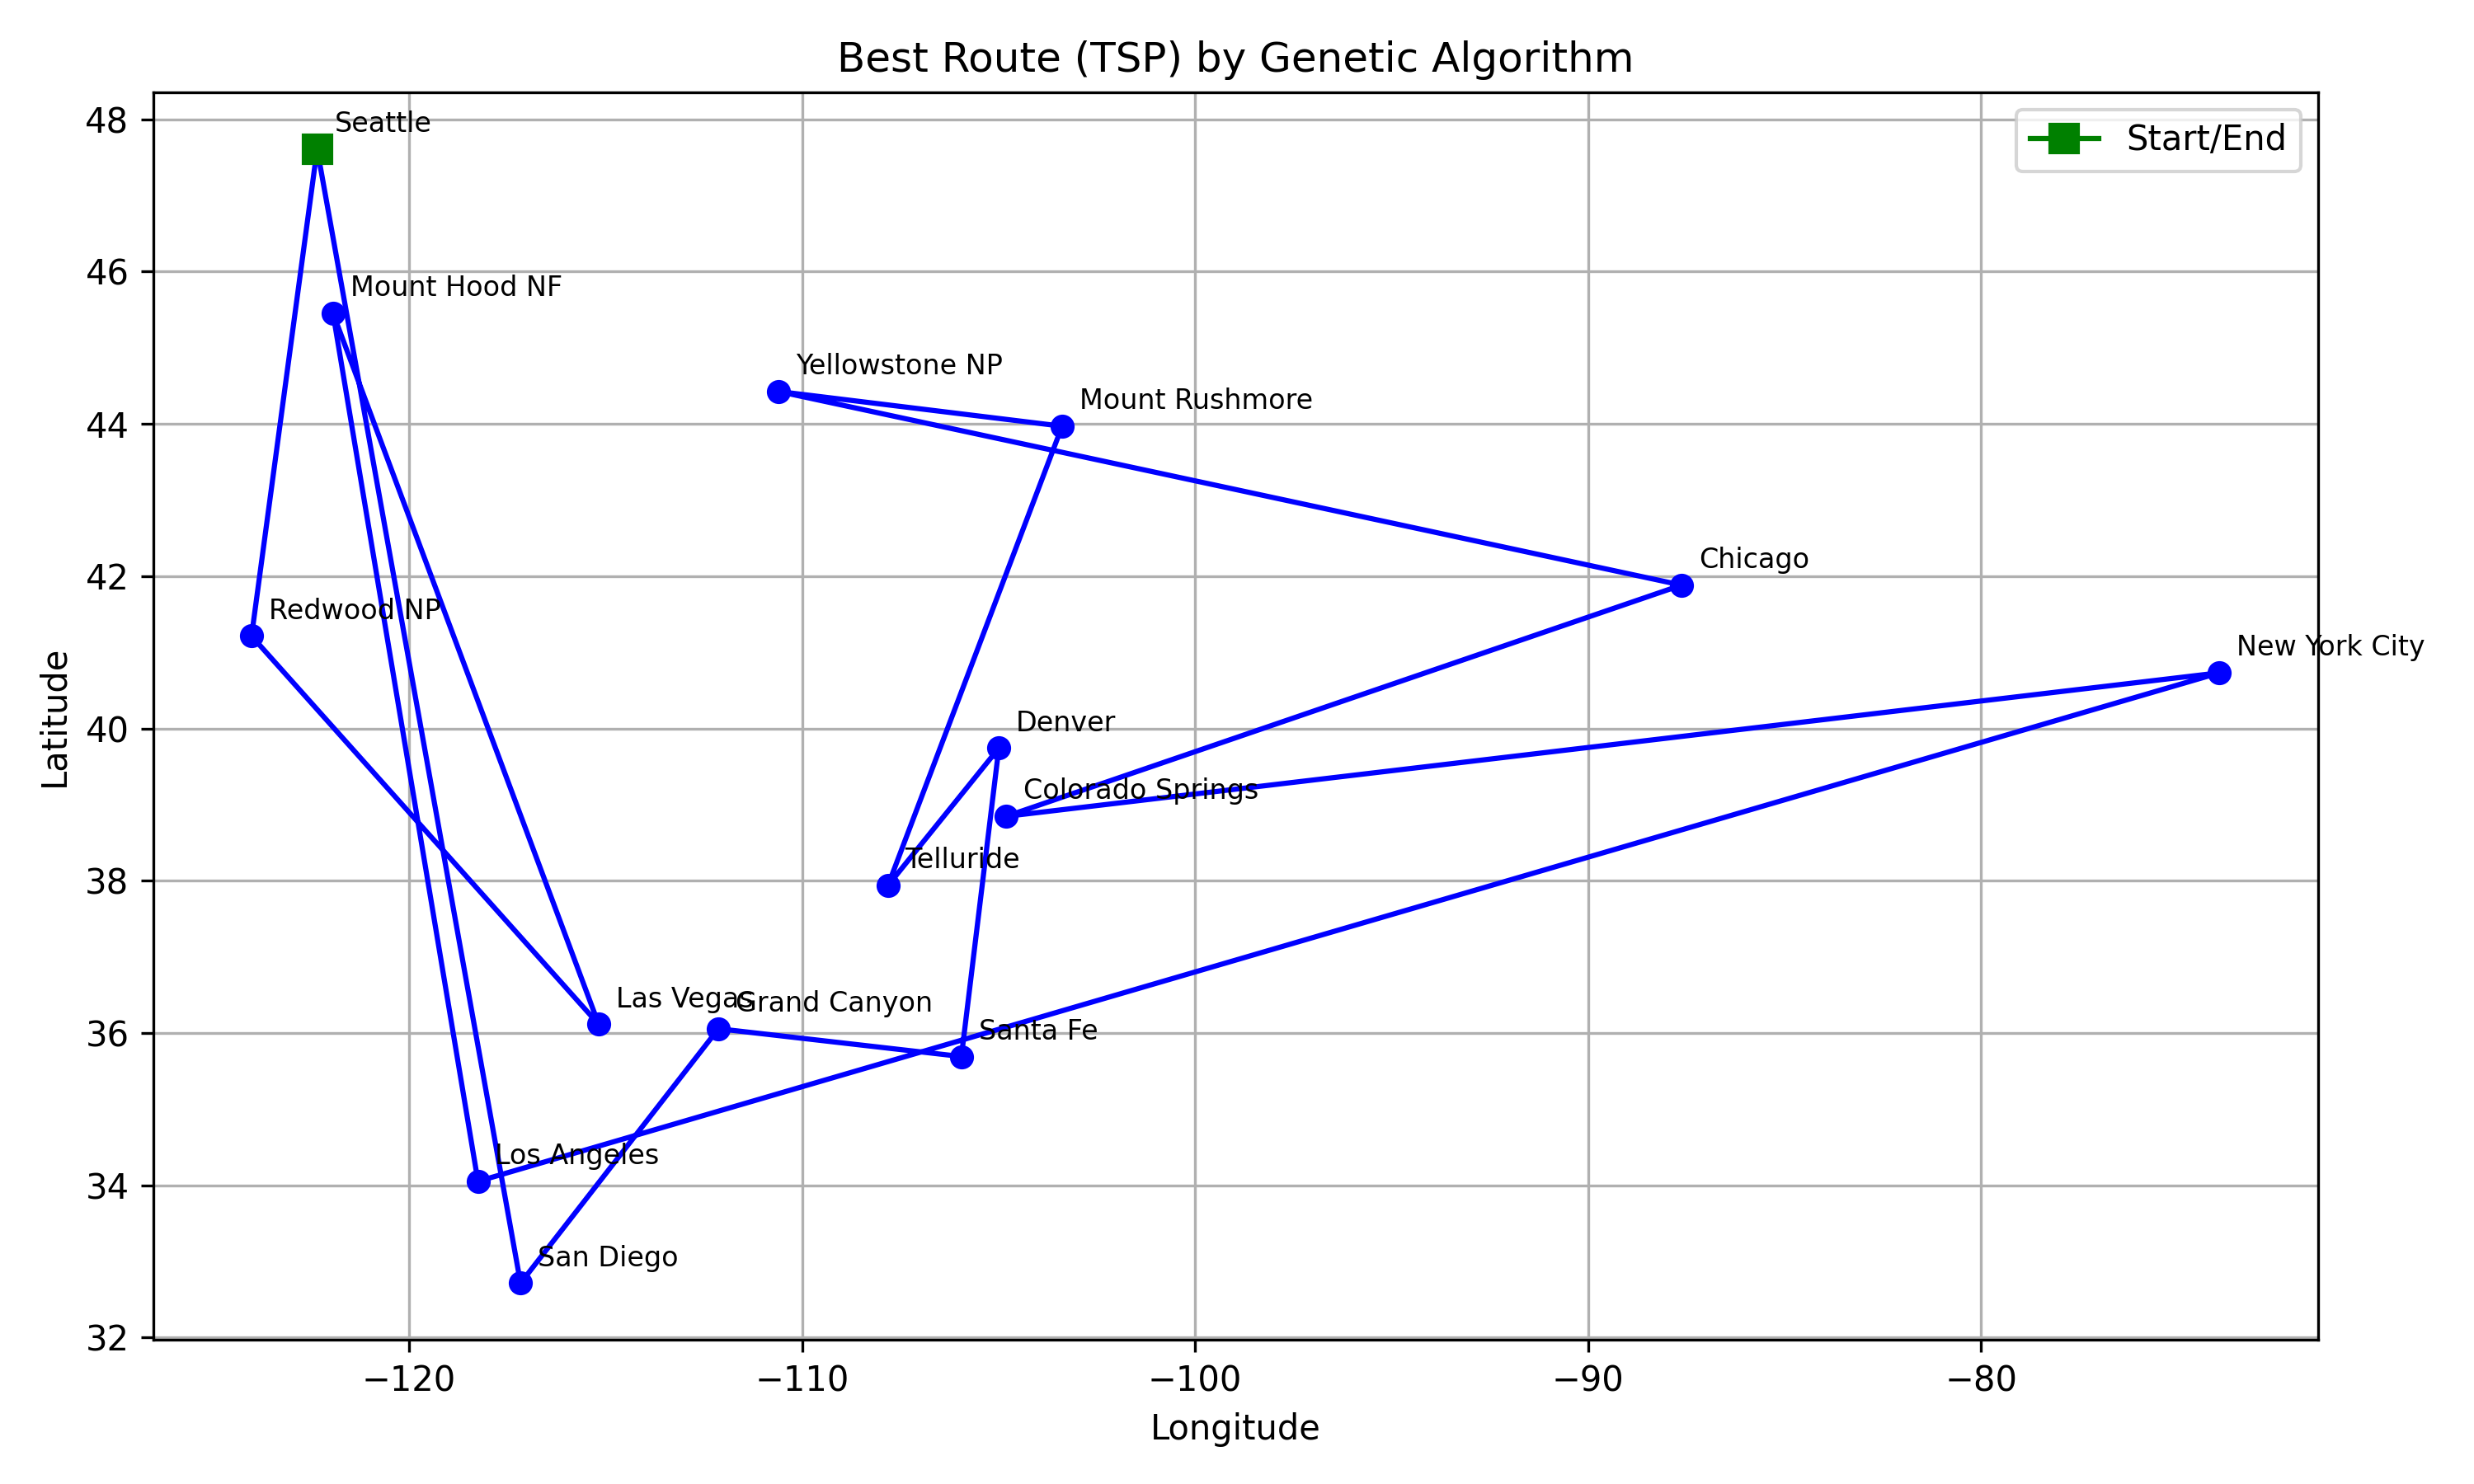
\includegraphics[width=0.85\textwidth]{media/best_route.png}
    \caption{Visualisasi Rute Terbaik Hasil Algoritma Genetika (\textit{Best Route})}
    \label{fig:best_route}
\end{figure}

\end{document}
